\documentclass[]{book}
\usepackage{lmodern}
\usepackage{amssymb,amsmath}
\usepackage{ifxetex,ifluatex}
\usepackage{fixltx2e} % provides \textsubscript
\ifnum 0\ifxetex 1\fi\ifluatex 1\fi=0 % if pdftex
  \usepackage[T1]{fontenc}
  \usepackage[utf8]{inputenc}
\else % if luatex or xelatex
  \ifxetex
    \usepackage{mathspec}
  \else
    \usepackage{fontspec}
  \fi
  \defaultfontfeatures{Ligatures=TeX,Scale=MatchLowercase}
\fi
% use upquote if available, for straight quotes in verbatim environments
\IfFileExists{upquote.sty}{\usepackage{upquote}}{}
% use microtype if available
\IfFileExists{microtype.sty}{%
\usepackage{microtype}
\UseMicrotypeSet[protrusion]{basicmath} % disable protrusion for tt fonts
}{}
\usepackage{hyperref}
\hypersetup{unicode=true,
            pdftitle={This is us: making CSAFE stronger each week},
            pdfauthor={CSAFE},
            pdfborder={0 0 0},
            breaklinks=true}
\urlstyle{same}  % don't use monospace font for urls
\usepackage{natbib}
\bibliographystyle{apalike}
\usepackage{color}
\usepackage{fancyvrb}
\newcommand{\VerbBar}{|}
\newcommand{\VERB}{\Verb[commandchars=\\\{\}]}
\DefineVerbatimEnvironment{Highlighting}{Verbatim}{commandchars=\\\{\}}
% Add ',fontsize=\small' for more characters per line
\usepackage{framed}
\definecolor{shadecolor}{RGB}{248,248,248}
\newenvironment{Shaded}{\begin{snugshade}}{\end{snugshade}}
\newcommand{\AlertTok}[1]{\textcolor[rgb]{0.94,0.16,0.16}{#1}}
\newcommand{\AnnotationTok}[1]{\textcolor[rgb]{0.56,0.35,0.01}{\textbf{\textit{#1}}}}
\newcommand{\AttributeTok}[1]{\textcolor[rgb]{0.77,0.63,0.00}{#1}}
\newcommand{\BaseNTok}[1]{\textcolor[rgb]{0.00,0.00,0.81}{#1}}
\newcommand{\BuiltInTok}[1]{#1}
\newcommand{\CharTok}[1]{\textcolor[rgb]{0.31,0.60,0.02}{#1}}
\newcommand{\CommentTok}[1]{\textcolor[rgb]{0.56,0.35,0.01}{\textit{#1}}}
\newcommand{\CommentVarTok}[1]{\textcolor[rgb]{0.56,0.35,0.01}{\textbf{\textit{#1}}}}
\newcommand{\ConstantTok}[1]{\textcolor[rgb]{0.00,0.00,0.00}{#1}}
\newcommand{\ControlFlowTok}[1]{\textcolor[rgb]{0.13,0.29,0.53}{\textbf{#1}}}
\newcommand{\DataTypeTok}[1]{\textcolor[rgb]{0.13,0.29,0.53}{#1}}
\newcommand{\DecValTok}[1]{\textcolor[rgb]{0.00,0.00,0.81}{#1}}
\newcommand{\DocumentationTok}[1]{\textcolor[rgb]{0.56,0.35,0.01}{\textbf{\textit{#1}}}}
\newcommand{\ErrorTok}[1]{\textcolor[rgb]{0.64,0.00,0.00}{\textbf{#1}}}
\newcommand{\ExtensionTok}[1]{#1}
\newcommand{\FloatTok}[1]{\textcolor[rgb]{0.00,0.00,0.81}{#1}}
\newcommand{\FunctionTok}[1]{\textcolor[rgb]{0.00,0.00,0.00}{#1}}
\newcommand{\ImportTok}[1]{#1}
\newcommand{\InformationTok}[1]{\textcolor[rgb]{0.56,0.35,0.01}{\textbf{\textit{#1}}}}
\newcommand{\KeywordTok}[1]{\textcolor[rgb]{0.13,0.29,0.53}{\textbf{#1}}}
\newcommand{\NormalTok}[1]{#1}
\newcommand{\OperatorTok}[1]{\textcolor[rgb]{0.81,0.36,0.00}{\textbf{#1}}}
\newcommand{\OtherTok}[1]{\textcolor[rgb]{0.56,0.35,0.01}{#1}}
\newcommand{\PreprocessorTok}[1]{\textcolor[rgb]{0.56,0.35,0.01}{\textit{#1}}}
\newcommand{\RegionMarkerTok}[1]{#1}
\newcommand{\SpecialCharTok}[1]{\textcolor[rgb]{0.00,0.00,0.00}{#1}}
\newcommand{\SpecialStringTok}[1]{\textcolor[rgb]{0.31,0.60,0.02}{#1}}
\newcommand{\StringTok}[1]{\textcolor[rgb]{0.31,0.60,0.02}{#1}}
\newcommand{\VariableTok}[1]{\textcolor[rgb]{0.00,0.00,0.00}{#1}}
\newcommand{\VerbatimStringTok}[1]{\textcolor[rgb]{0.31,0.60,0.02}{#1}}
\newcommand{\WarningTok}[1]{\textcolor[rgb]{0.56,0.35,0.01}{\textbf{\textit{#1}}}}
\usepackage{longtable,booktabs}
\usepackage{graphicx,grffile}
\makeatletter
\def\maxwidth{\ifdim\Gin@nat@width>\linewidth\linewidth\else\Gin@nat@width\fi}
\def\maxheight{\ifdim\Gin@nat@height>\textheight\textheight\else\Gin@nat@height\fi}
\makeatother
% Scale images if necessary, so that they will not overflow the page
% margins by default, and it is still possible to overwrite the defaults
% using explicit options in \includegraphics[width, height, ...]{}
\setkeys{Gin}{width=\maxwidth,height=\maxheight,keepaspectratio}
\IfFileExists{parskip.sty}{%
\usepackage{parskip}
}{% else
\setlength{\parindent}{0pt}
\setlength{\parskip}{6pt plus 2pt minus 1pt}
}
\setlength{\emergencystretch}{3em}  % prevent overfull lines
\providecommand{\tightlist}{%
  \setlength{\itemsep}{0pt}\setlength{\parskip}{0pt}}
\setcounter{secnumdepth}{5}
% Redefines (sub)paragraphs to behave more like sections
\ifx\paragraph\undefined\else
\let\oldparagraph\paragraph
\renewcommand{\paragraph}[1]{\oldparagraph{#1}\mbox{}}
\fi
\ifx\subparagraph\undefined\else
\let\oldsubparagraph\subparagraph
\renewcommand{\subparagraph}[1]{\oldsubparagraph{#1}\mbox{}}
\fi

%%% Use protect on footnotes to avoid problems with footnotes in titles
\let\rmarkdownfootnote\footnote%
\def\footnote{\protect\rmarkdownfootnote}

%%% Change title format to be more compact
\usepackage{titling}

% Create subtitle command for use in maketitle
\providecommand{\subtitle}[1]{
  \posttitle{
    \begin{center}\large#1\end{center}
    }
}

\setlength{\droptitle}{-2em}

  \title{This is us: making CSAFE stronger each week}
    \pretitle{\vspace{\droptitle}\centering\huge}
  \posttitle{\par}
    \author{CSAFE}
    \preauthor{\centering\large\emph}
  \postauthor{\par}
      \predate{\centering\large\emph}
  \postdate{\par}
    \date{2019-09-12}

\usepackage{booktabs}
\usepackage{amsthm}
\makeatletter
\def\thm@space@setup{%
  \thm@preskip=8pt plus 2pt minus 4pt
  \thm@postskip=\thm@preskip
}
\makeatother

\begin{document}
\maketitle

{
\setcounter{tocdepth}{1}
\tableofcontents
}
\hypertarget{prerequisites}{%
\chapter{Prerequisites}\label{prerequisites}}

This is a \emph{sample} book written in \textbf{Markdown}. You can use anything that Pandoc's Markdown supports, e.g., a math equation \(a^2 + b^2 = c^2\).

The \textbf{bookdown} package can be installed from CRAN or Github:

\begin{Shaded}
\begin{Highlighting}[]
\KeywordTok{install.packages}\NormalTok{(}\StringTok{"bookdown"}\NormalTok{)}
\CommentTok{# or the development version}
\CommentTok{# devtools::install_github("rstudio/bookdown")}
\end{Highlighting}
\end{Shaded}

Remember each Rmd file contains one and only one chapter, and a chapter is defined by the first-level heading \texttt{\#}.

To compile this example to PDF, you need XeLaTeX. You are recommended to install TinyTeX (which includes XeLaTeX): \url{https://yihui.name/tinytex/}.

\hypertarget{intro}{%
\chapter{Introduction}\label{intro}}

This section will become the section for the administrative updates/organization once we have figured out how to use all of the bookdown features for our purposes.

You can label chapter and section titles using \texttt{\{\#label\}} after them, e.g., we can reference Chapter \ref{intro}. If you do not manually label them, there will be automatic labels anyway, e.g., Chapter \ref{glass}.

Figures and tables with captions will be placed in \texttt{figure} and \texttt{table} environments, respectively.

\begin{Shaded}
\begin{Highlighting}[]
\KeywordTok{par}\NormalTok{(}\DataTypeTok{mar =} \KeywordTok{c}\NormalTok{(}\DecValTok{4}\NormalTok{, }\DecValTok{4}\NormalTok{, }\FloatTok{.1}\NormalTok{, }\FloatTok{.1}\NormalTok{))}
\KeywordTok{plot}\NormalTok{(pressure, }\DataTypeTok{type =} \StringTok{'b'}\NormalTok{, }\DataTypeTok{pch =} \DecValTok{19}\NormalTok{)}
\end{Highlighting}
\end{Shaded}

\begin{figure}

{\centering 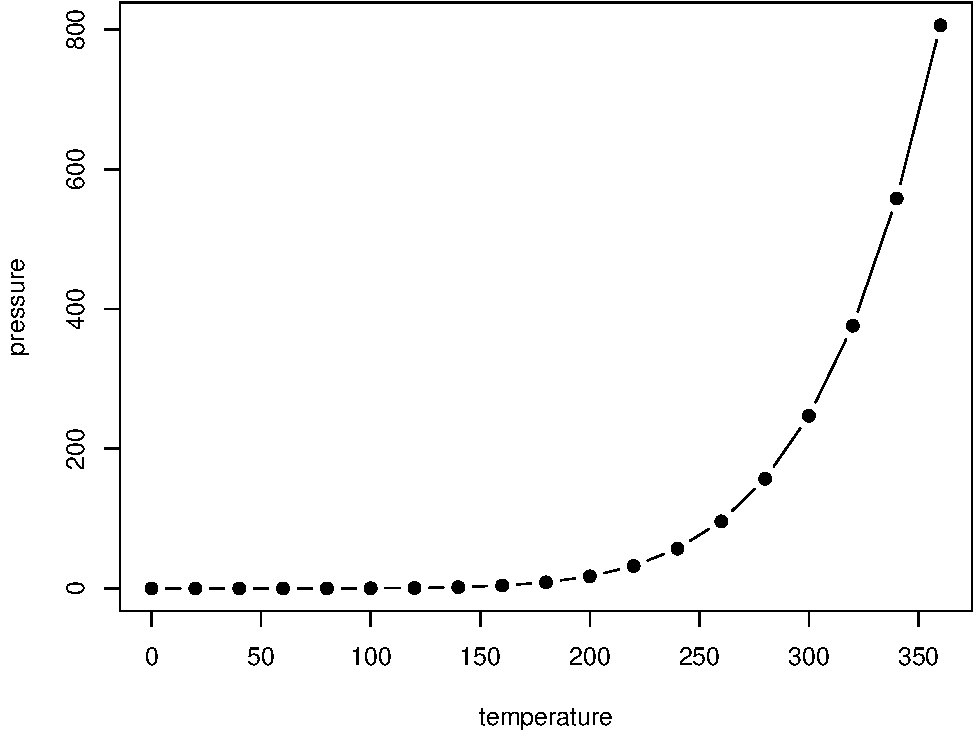
\includegraphics[width=0.8\linewidth]{bookdown-demo_files/figure-latex/nice-fig-1} 

}

\caption{Here is a nice figure!}\label{fig:nice-fig}
\end{figure}

Reference a figure by its code chunk label with the \texttt{fig:} prefix, e.g., see Figure \ref{fig:nice-fig}. Similarly, you can reference tables generated from \texttt{knitr::kable()}, e.g., see Table \ref{tab:nice-tab}.

\begin{Shaded}
\begin{Highlighting}[]
\NormalTok{knitr}\OperatorTok{::}\KeywordTok{kable}\NormalTok{(}
  \KeywordTok{head}\NormalTok{(iris, }\DecValTok{20}\NormalTok{), }\DataTypeTok{caption =} \StringTok{'Here is a nice table!'}\NormalTok{,}
  \DataTypeTok{booktabs =} \OtherTok{TRUE}
\NormalTok{)}
\end{Highlighting}
\end{Shaded}

\begin{table}[t]

\caption{\label{tab:nice-tab}Here is a nice table!}
\centering
\begin{tabular}{rrrrl}
\toprule
Sepal.Length & Sepal.Width & Petal.Length & Petal.Width & Species\\
\midrule
5.1 & 3.5 & 1.4 & 0.2 & setosa\\
4.9 & 3.0 & 1.4 & 0.2 & setosa\\
4.7 & 3.2 & 1.3 & 0.2 & setosa\\
4.6 & 3.1 & 1.5 & 0.2 & setosa\\
5.0 & 3.6 & 1.4 & 0.2 & setosa\\
\addlinespace
5.4 & 3.9 & 1.7 & 0.4 & setosa\\
4.6 & 3.4 & 1.4 & 0.3 & setosa\\
5.0 & 3.4 & 1.5 & 0.2 & setosa\\
4.4 & 2.9 & 1.4 & 0.2 & setosa\\
4.9 & 3.1 & 1.5 & 0.1 & setosa\\
\addlinespace
5.4 & 3.7 & 1.5 & 0.2 & setosa\\
4.8 & 3.4 & 1.6 & 0.2 & setosa\\
4.8 & 3.0 & 1.4 & 0.1 & setosa\\
4.3 & 3.0 & 1.1 & 0.1 & setosa\\
5.8 & 4.0 & 1.2 & 0.2 & setosa\\
\addlinespace
5.7 & 4.4 & 1.5 & 0.4 & setosa\\
5.4 & 3.9 & 1.3 & 0.4 & setosa\\
5.1 & 3.5 & 1.4 & 0.3 & setosa\\
5.7 & 3.8 & 1.7 & 0.3 & setosa\\
5.1 & 3.8 & 1.5 & 0.3 & setosa\\
\bottomrule
\end{tabular}
\end{table}

You can write citations, too. For example, we are using the \textbf{bookdown} package \citep{R-bookdown} in this sample book, which was built on top of R Markdown and \textbf{knitr} \citep{xie2015}.

\hypertarget{bullets}{%
\chapter{Project CC: Bullets and Cartridge Cases}\label{bullets}}

For both bullets and cartridge cases we are dealing with several inter-related aspects, that we want to address independently.

Those are:

\begin{enumerate}
\def\labelenumi{\arabic{enumi}.}
\item
  data collection
\item
  computational tools
\item
  similarity scores

  \begin{enumerate}
  \def\labelenumii{\arabic{enumii}.}
  \item
    for bullet lands:

    \begin{enumerate}
    \def\labelenumiii{\alph{enumiii}.}
    \tightlist
    \item
      crosscut identification
    \item
      groove location
    \item
      curvature removal
    \item
      alignment of signatures
    \item
      feature extraction
    \item
      matching with trained Random Forest
    \end{enumerate}
  \item
    for breech faces
  \end{enumerate}
\item
  analysis of results
\item
  communication of results and methods
\end{enumerate}

\hypertarget{data-collection}{%
\section{Data Collection}\label{data-collection}}

\hypertarget{lapd}{%
\subsection{LAPD}\label{lapd}}

All bullets are collected by Srinivasan Rathinam, LAPD.

\hypertarget{main-study}{%
\subsubsection{Main study}\label{main-study}}

4 bullets per barrel for 626 Beretta 92 F/FS firearms , ammunition used are 9 mm Luger Winchester 115 grain with a Copper surface.

scans are on Raven.

evaluation: Yawei is going to work through all 626 barrels of knowns to assess similarity scores

\begin{figure}

{\centering 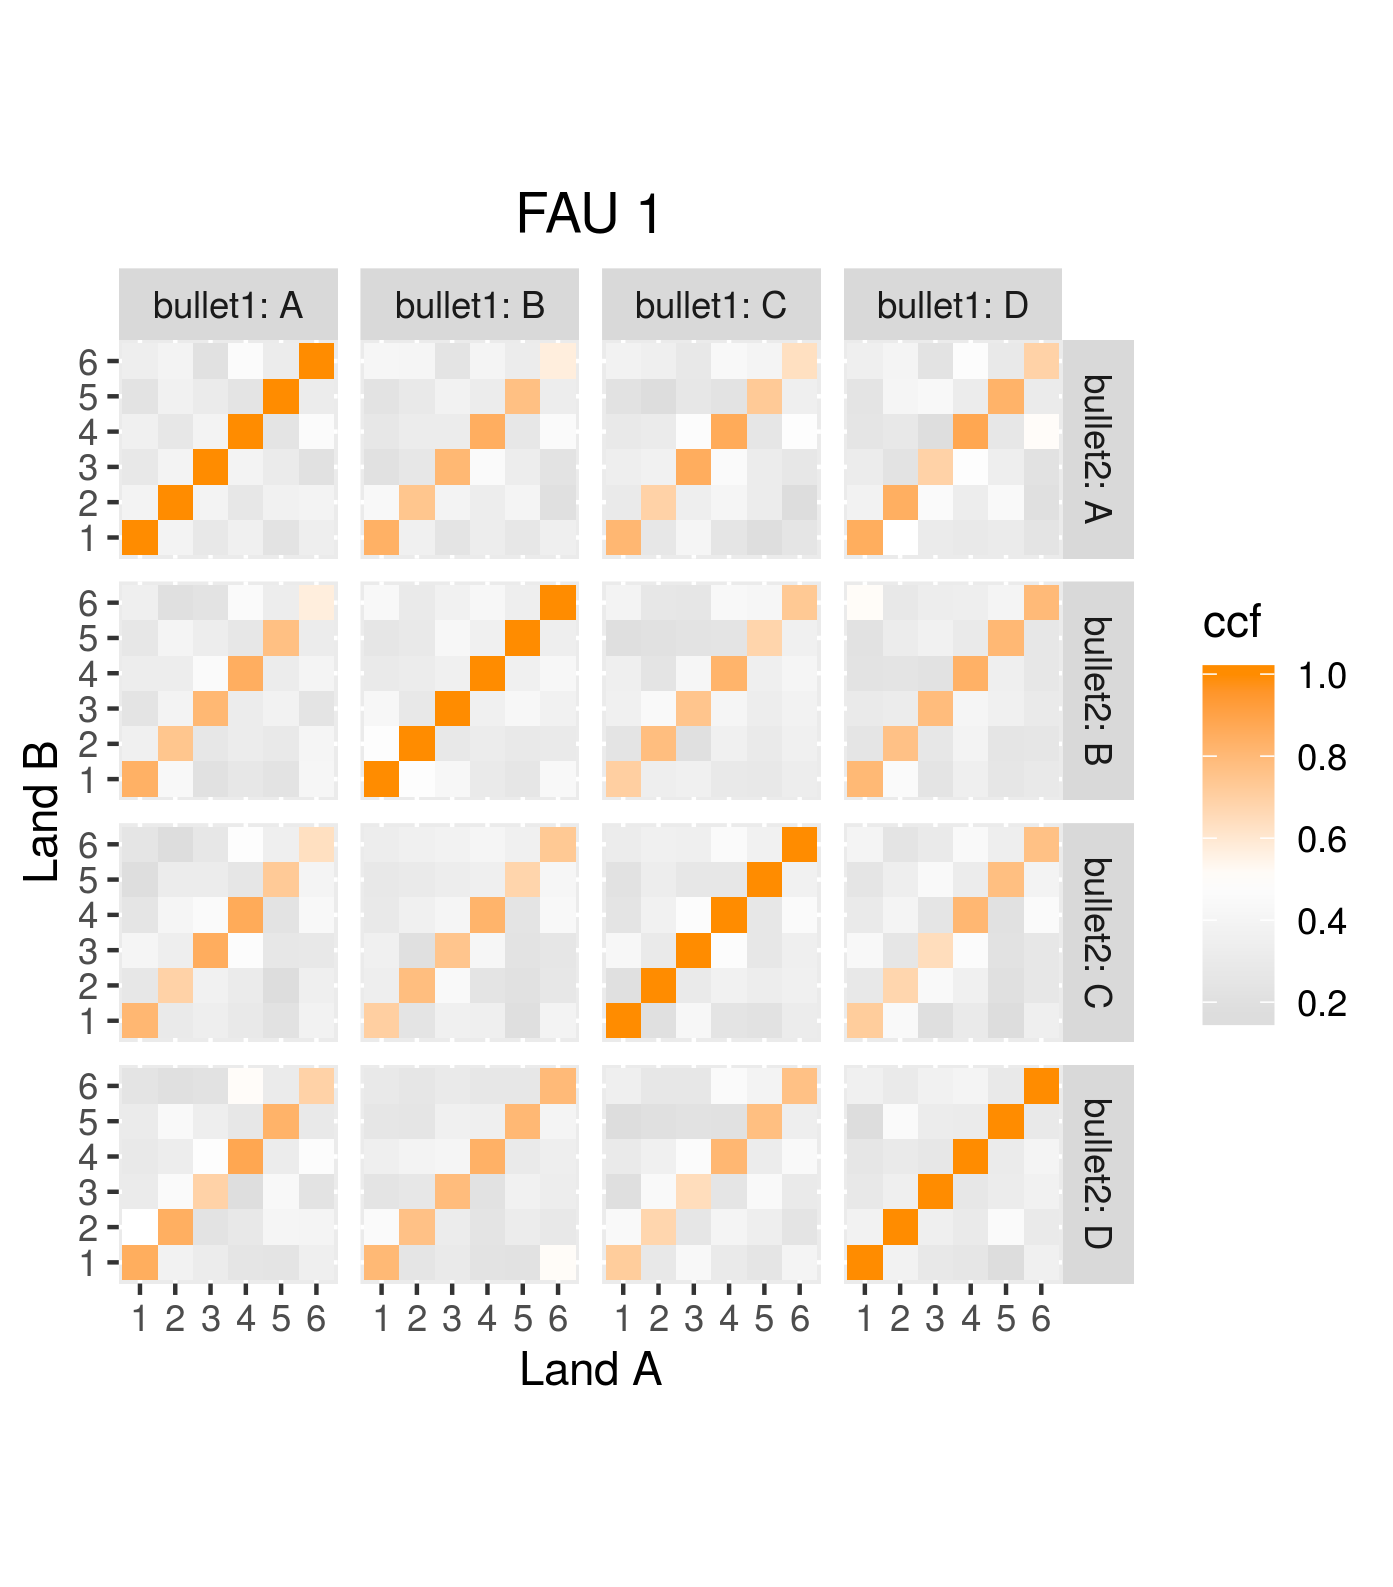
\includegraphics[width=0.5\linewidth]{images/yawei/results-FAU-1} 

}

\caption{Results from assessing scans of barrel FAU 1 similarity.}\label{fig:unnamed-chunk-3}
\end{figure}

\begin{figure}

{\centering 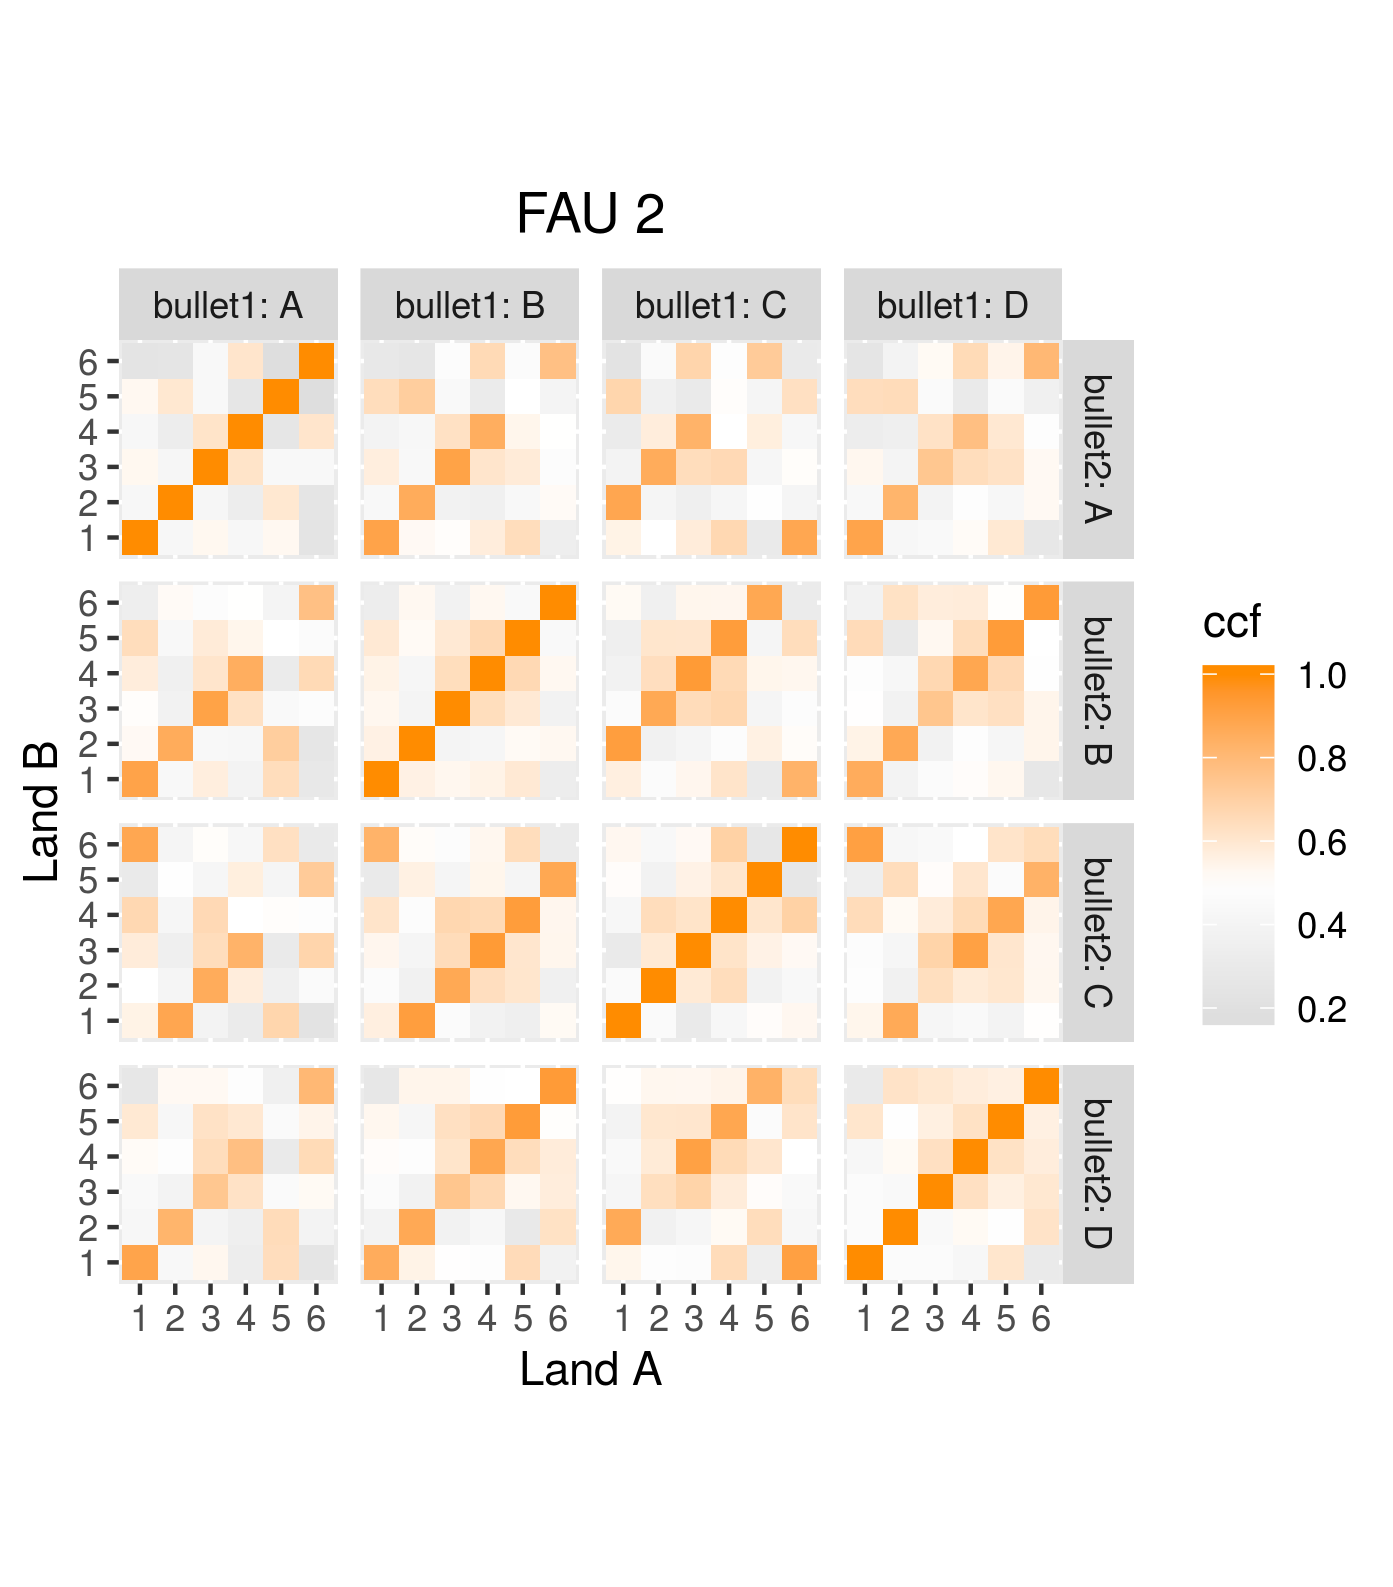
\includegraphics[width=0.5\linewidth]{images/yawei/results-FAU-2} 

}

\caption{Results from assessing scans of barrel FAU 2 similarity.}\label{fig:unnamed-chunk-4}
\end{figure}

Why some of the cases failed? (181/626 = 30\%)

\texttt{x3p\_crosscut\_optimize()} failed to find the positions to get cross cut for some lands.

\begin{figure}

{\centering 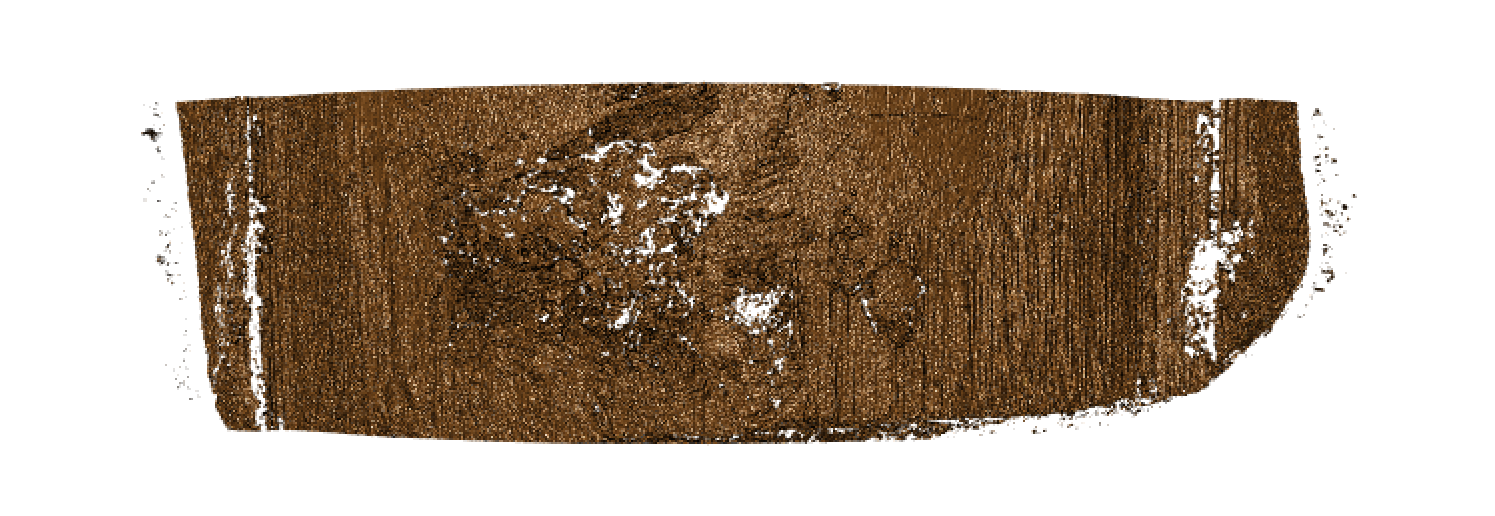
\includegraphics[width=0.5\linewidth]{images/yawei/lapd-FAU-3-Bullet-A-land-6} 

}

\caption{Land scan for barrel FAU 3 bullet A land 6.}\label{fig:unnamed-chunk-5}
\end{figure}

\begin{figure}

{\centering 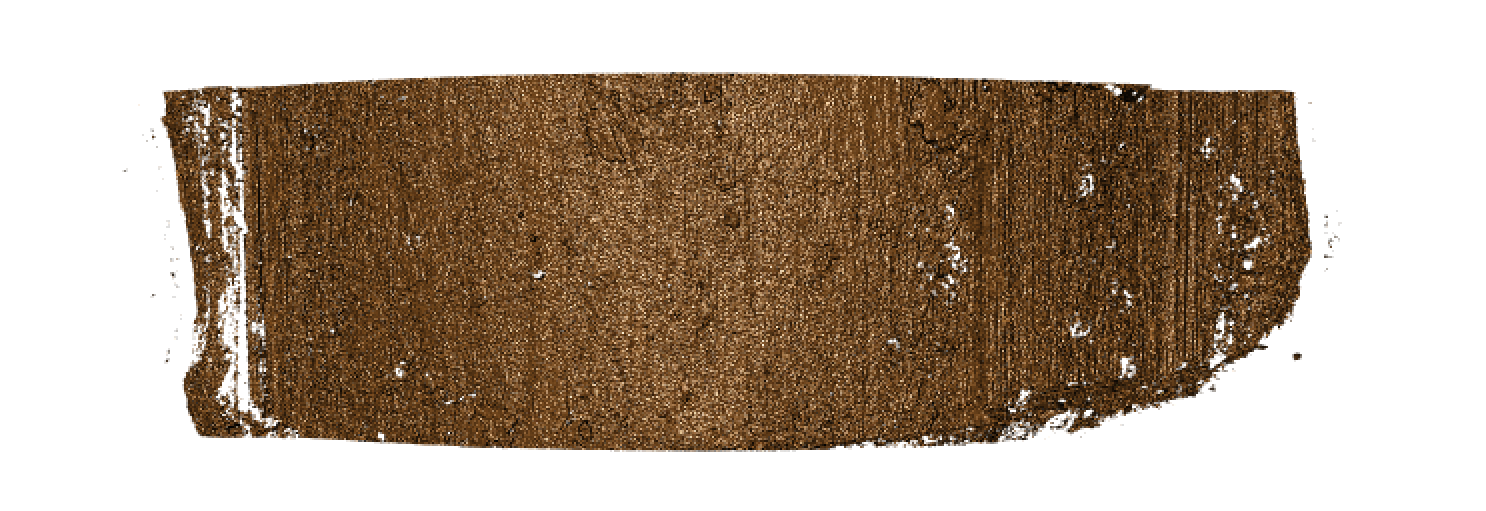
\includegraphics[width=0.5\linewidth]{images/yawei/lapd-FAU-4-Bullet-C-land-5} 

}

\caption{Land scan for barrel FAU 4 bullet C land 5.}\label{fig:unnamed-chunk-6}
\end{figure}

\begin{figure}

{\centering 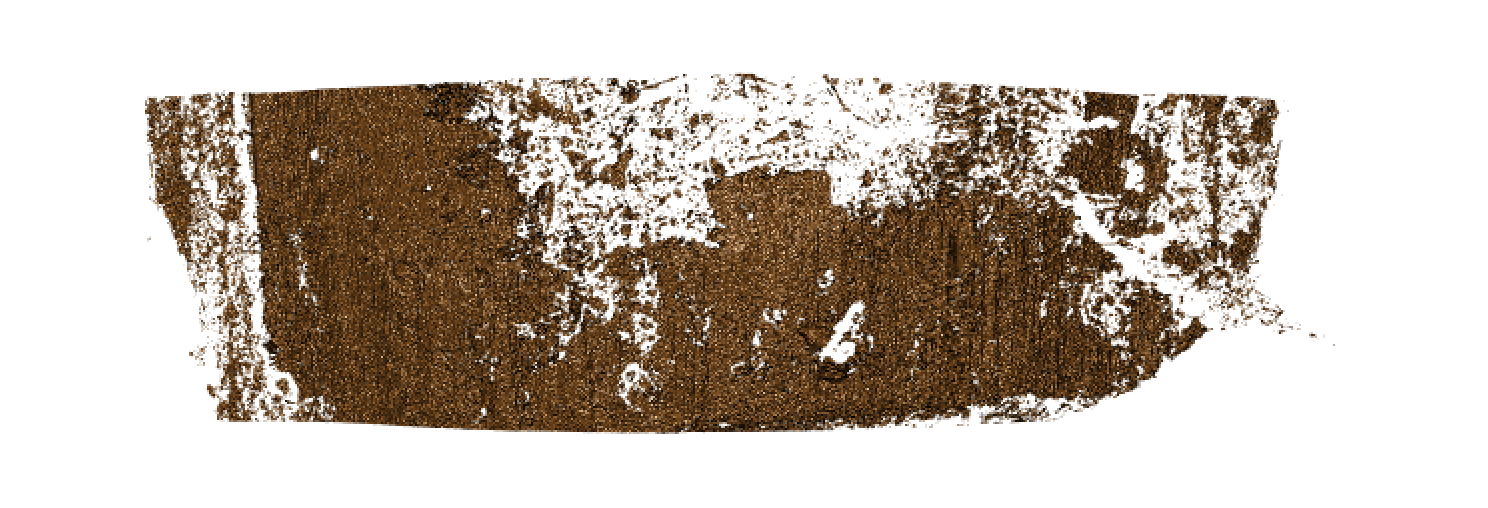
\includegraphics[width=0.5\linewidth]{images/yawei/lapd-FAU-5-Bullet-B-land-5} 

}

\caption{Land scan for barrel FAU 5 bullet B land 5.}\label{fig:unnamed-chunk-7}
\end{figure}

Manual indentification of grooves now\ldots{}

\hypertarget{follow-up-study}{%
\subsubsection{follow-up study}\label{follow-up-study}}

4 bullets per barrel for 96 of the original 626 Beretta firearms using different ammunition

bullets are being scanned

\hypertarget{hamby-sets}{%
\subsection{Hamby Sets}\label{hamby-sets}}

Scans for Hamby Sets 10, 36, 44, and 224

Scans for 3 replicates of clones for Hamby 224

\hypertarget{houston-tests}{%
\subsection{Houston Tests}\label{houston-tests}}

contact: Melissa Nally, Houston FSI

\hypertarget{pre-study}{%
\subsubsection{Pre-study}\label{pre-study}}

3 kits with 23 bullets each

\begin{figure}

{\centering 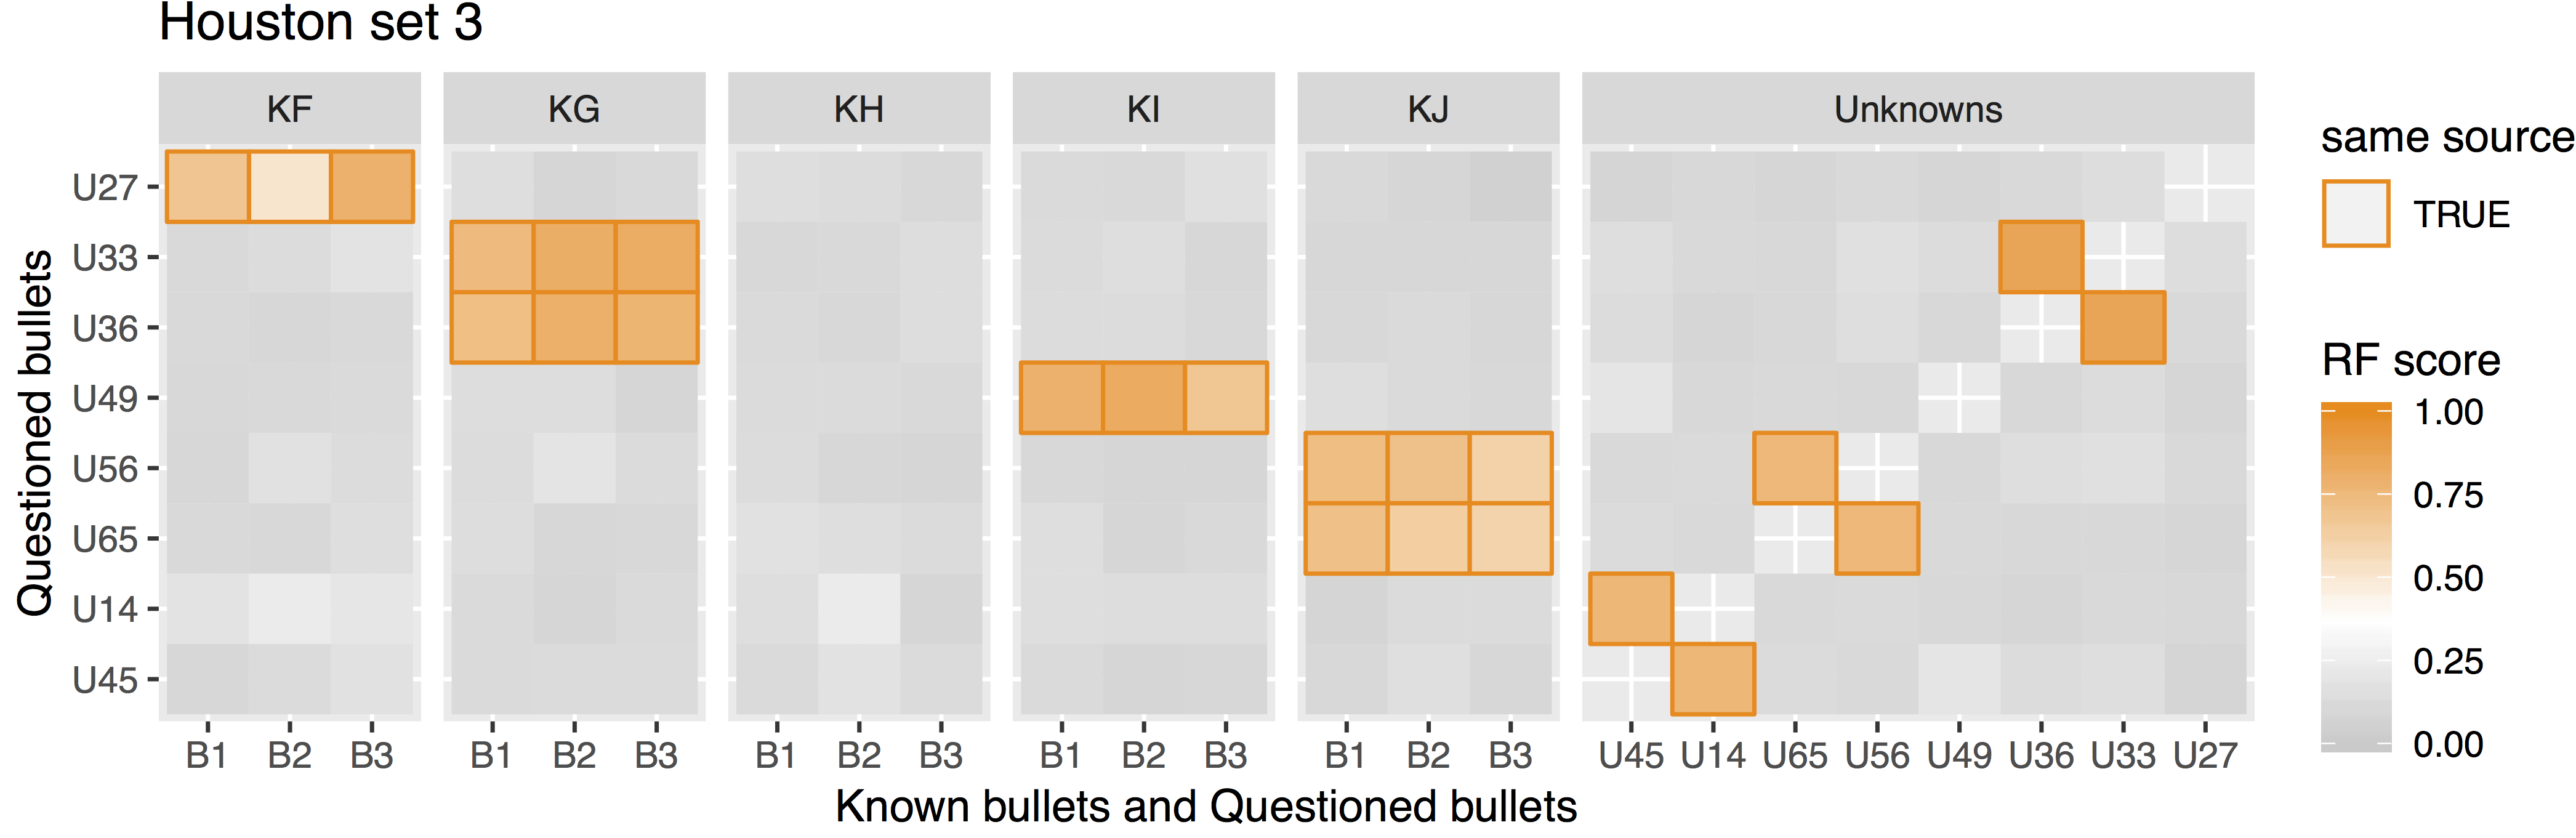
\includegraphics[width=58.11in]{images/bullets/houston-pre-set3} 

}

\caption{Bullet-to-bullet similarity scores for questioned bullets (y-axis) compared to all other bullets of the test set (x-axis).}\label{fig:unnamed-chunk-8}
\end{figure}

evaluation included in submission to JFI

\hypertarget{study}{%
\subsubsection{Study}\label{study}}

4 kits with 20 bullets each

scans done, evaluation finished, some scans of doubtful quality

\hypertarget{houston-persistence}{%
\subsection{Houston Persistence}\label{houston-persistence}}

contact: Melissa Nally, Houston FSI

8 barrels with 40 fired bullets each

\hypertarget{st-louis-persistence}{%
\subsection{St Louis persistence}\label{st-louis-persistence}}

contact: Steve Kramer, St Louis PD

2 barrels with 192 fired bullets each (2 bullets collected every 25 shots)

\hypertarget{dfsc-cartridge-cases}{%
\subsection{DFSC Cartridge cases}\label{dfsc-cartridge-cases}}

Breech face data for knowns are scanned and available on a private github repository

evaluation

\hypertarget{computational-tools}{%
\section{Computational Tools}\label{computational-tools}}

\hypertarget{x3ptools}{%
\subsection{x3ptools}\label{x3ptools}}

\texttt{x3ptools} is an R package for working with files in x3p format. x3p is an ISO standard for describing 3d topographic surface measurements.
\texttt{x3ptools} is available on CRAN, i.e.~can be installed with the command \texttt{install.packages("x3ptools")}. The development version is available from github. Installation instructions and basic usage can be found at \url{https://heike.github.io/x3ptools/}

\hypertarget{bulletxtrctr}{%
\subsection{bulletxtrctr}\label{bulletxtrctr}}

\texttt{bulletxtrctr} is a developmental R package available from github (see \url{https://heike.github.io/bulletxtrctr/}) that allows an assessment of similarity scores using the data extraction pipeline described in \citet{aoas}.

\hypertarget{groovefinder}{%
\subsection{grooveFinder}\label{groovefinder}}

\texttt{grooveFinder} is a developmental R package providing different methods for identifying the location of grooves in scans of bullets.
Installation instructions and some basic usage can be found at \url{https://heike.github.io/grooveFinder/}

\hypertarget{similarity-scores}{%
\section{Similarity Scores}\label{similarity-scores}}

\hypertarget{bullet-lands}{%
\subsection{Bullet Lands}\label{bullet-lands}}

\hypertarget{approaches-to-identify-groove-locations}{%
\subsubsection{Approaches to identify groove locations}\label{approaches-to-identify-groove-locations}}

\hypertarget{hough-transform-method-for-identifying-grooves}{%
\paragraph{Hough Transform Method for Identifying Grooves}\label{hough-transform-method-for-identifying-grooves}}

Charlotte 9/5/19 Update:

Will fill in with more detail later

\textbf{Current Goals}:
- Iron-out issues with consistency of units with \texttt{get\_hough\_grooves}. I believe there are some issues translating from the 2-d visualization to the 3-d visualization that might have to do with inconsistent unit inputs? For Example

\begin{figure}

{\centering 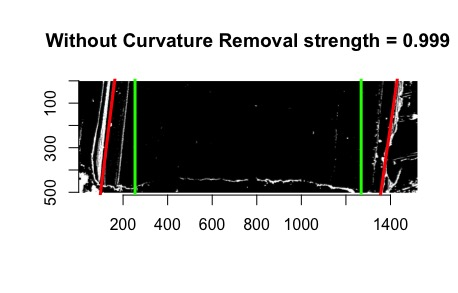
\includegraphics[width=0.5\linewidth]{images/bullets/Hough_project/br411_2d} 

}

\caption{2-dimensional visualization of example bullet br411 with .999 strength threshold}\label{fig:unnamed-chunk-9}
\end{figure}

\begin{figure}

{\centering 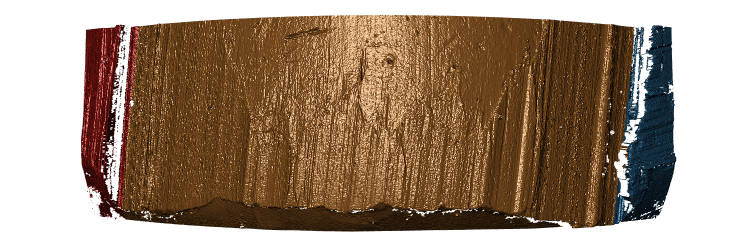
\includegraphics[width=0.5\linewidth]{images/bullets/Hough_project/br411_3d} 

}

\caption{3-dimensional visualization of example bullet br411 with .999 strength threshold}\label{fig:unnamed-chunk-10}
\end{figure}

So either somethin is wrong with \texttt{get\_mask\_hough} or something is funky with the units.

\begin{itemize}
\item
  Also need to think of including a sort of rounding component where lines with slopes that are practically infinite can be viewed as a vertical line
\item
  Compare Hough results with manual identification using score calculations from Kiegan.
\item
  Write up results in Hough Groove Paper (It's coming I promise)

  \begin{itemize}
  \tightlist
  \item
    Create graphical images to explain line selection method
  \item
    Include 2-d and 3-d visualizations of Hough groove area identifications
  \item
    Include crosscut visualization and comparison in results
  \end{itemize}
\end{itemize}

\hypertarget{lasso-method}{%
\paragraph{LASSO Method}\label{lasso-method}}

A paper is in preparation for submission to Forensic Science International describing this method (\texttt{get\_grooves\_lassofull} in \texttt{grooveFinder}), as well as the Bayesian changepoint method (\texttt{get\_grooves\_bcp}).

\hypertarget{robust-loess-method}{%
\paragraph{Robust LOESS Method}\label{robust-loess-method}}

A paper submitted to the Journal of Forensic Science is waiting for peer review response to the first round of revisions.

\hypertarget{cartridge-cases}{%
\subsection{Cartridge Cases}\label{cartridge-cases}}

\hypertarget{congruent-matching-cells-cmc-algorithm-for-comparing-cartridge-case-breech-face-impressions}{%
\subsubsection{Congruent Matching Cells (CMC) algorithm for comparing cartridge case breech face impressions}\label{congruent-matching-cells-cmc-algorithm-for-comparing-cartridge-case-breech-face-impressions}}

Joe 9/5/19 Update: Dealing with missing values in the x3p scans continues to be an issue. The Fast Fourier Transform method for calculating cross-correlation can't handle missing data in an image, so we've attempted a few ``fixes'' that haven't necessarily turned out as well as expected. One idea we had was to replace the NA values in a cell with the average pixel value. However, this is artificially introducing a signal where before there was none. This can (and demonstrably has) led to inflated/incorrect correlations between cells that shouldn't have much at all in common. Unfortunately, this may be the only solution if we still wish to adhere to the CMC algorithm as described in Song et al. (2015). One improvement that I've implemented is to ``crop out'' the rows and columns of an image that only contain NAs. This at least means that we've weakened the strength of the artificial signal relative to the breechface's signal.

Below is a series of images that illustrate how we might compare a cell in one image to a region of another image.

\begin{figure}

{\centering 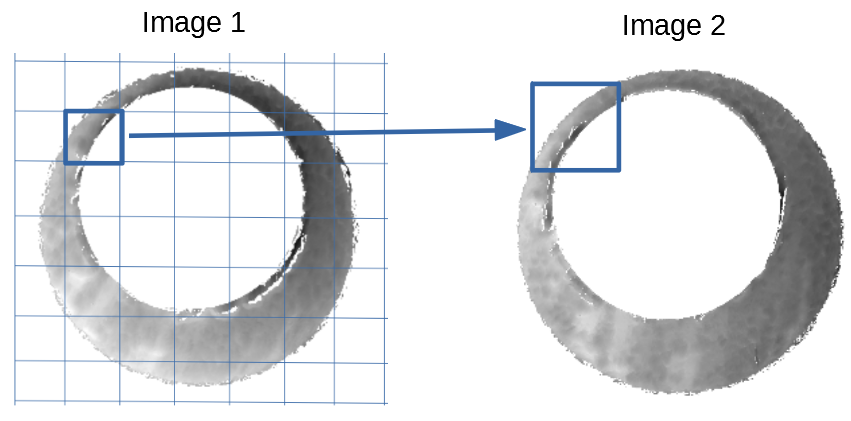
\includegraphics[width=0.5\linewidth]{images/cartridge_cases/im1_im2_cellComparison} 

}

\caption{Comparing a cell in image 1 to a larger region in image 2. We wish to find the translations of the image 1 cell that yield the highest correlation within the image 2 region.}\label{fig:unnamed-chunk-11}
\end{figure}

For the sake of an example, let's focus on the blue outlined cell in image 1. Our goal is to use the image 1 cell to ``search'' a corresponding larger region in image 2 for the horizontal/vertical translations needed to produce the highest correlation. Below is a zoomed-in version of the blue outlined image 1 cell on the left and the larger image 2 region (approximately: I made the gridded image above by-hand outside of R while the images below are from R). The image 1 cell may look larger than the image 2 region, but we can see from the axes that the image 2 region is indeed larger. Any white pixels in the two images are NA values that need to be dealt with in some way before we can use FFTs to calculate the cross-correlation.

\begin{figure}

{\centering 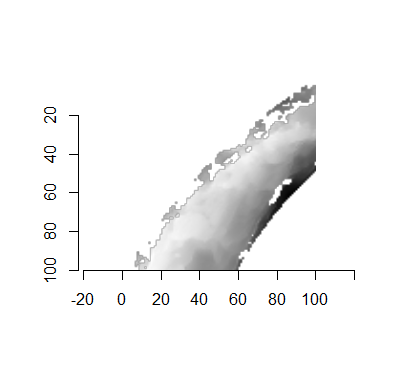
\includegraphics[width=0.5\linewidth]{images/cartridge_cases/im1_split} 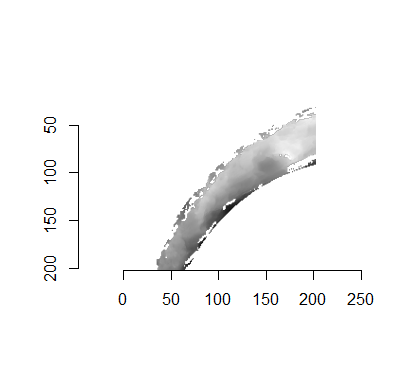
\includegraphics[width=0.5\linewidth]{images/cartridge_cases/im2_split} 

}

\caption{(Left) A cell from image 1. (Right) A region from image 2 centered in the same location as the image 1 cell, yet quadruple the area.}\label{fig:unnamed-chunk-12}
\end{figure}

As already discussed above, one ``solution'' is to replace the NA values with the average pixel value of each image. However, to avoid creating a stronger artificial signal than necessary, we can crop-out the NA rows and columns from the two images above. Below is the cropped version of the two images. The cropping doesn't produce signficantly different images in this case, but you could imagine other examples in which a cell has captured only small amount of breechface in the corner. Such examples are fairly common and cropping signficantly changes the resulting correlation values.

\begin{figure}

{\centering 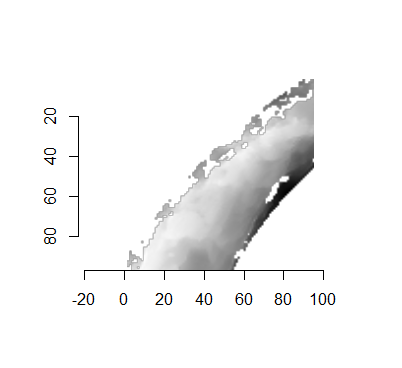
\includegraphics[width=0.5\linewidth]{images/cartridge_cases/im1_splitFilteredCropped} 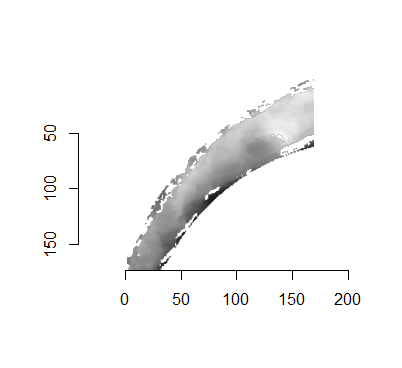
\includegraphics[width=0.5\linewidth]{images/cartridge_cases/im2_splitFilteredCropped} 

}

\caption{The same images as above after cropping NA rows/columns.}\label{fig:unnamed-chunk-13}
\end{figure}

The last step before calculating correlation for these cells is to replace the remaining NAs with the average pixel value. This is shown below.

\begin{figure}

{\centering 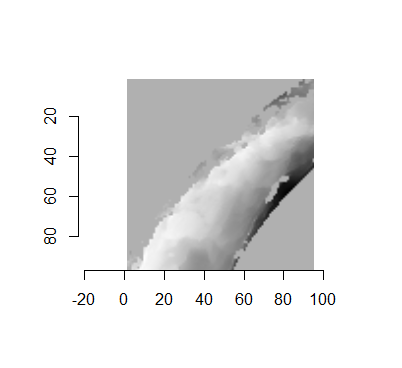
\includegraphics[width=0.5\linewidth]{images/cartridge_cases/im1_splitShifted} 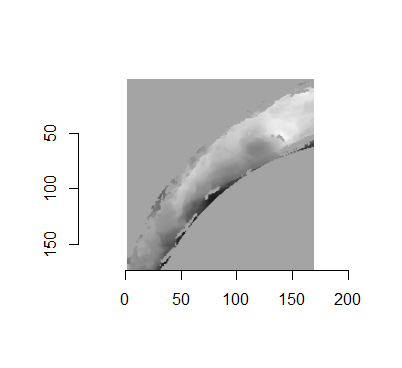
\includegraphics[width=0.5\linewidth]{images/cartridge_cases/im2_splitShifted} 

}

\caption{The NA-cropped images with remaining NAs replaced with the image's average pixel values.}\label{fig:unnamed-chunk-14}
\end{figure}

The cross-correlation is then calculated between these two images via a standard fast fourier transform process (see \href{http://mathworld.wolfram.com/Cross-CorrelationTheorem.html}{Cross-Correlation Theorem}). The benefit of using such a process is that (as the name suggests) it's faster than calculating the raw correlation between the two images. Also, the translations that produce the highest correlation between the image 1 cell and the image 2 region fall out of the calculation for free.

This pre-processing/cross-correlation calculation procedure is repeated for every cell in image 1 that contains breech face impression. Because it is not valid to assume that the two images are rotationally aligned by default, we perform the same procedure repeatedly while rotating image 2. Currently, we perform a ``rough'' grid search of \(\theta \in [-177.5,180]\) by increments of \(2.5^{\circ}\). Theoretically, the final results tell us how we need to horizontally/vertically translate and rotate the two images to be correctly aligned.

\hypertarget{congruent-matching-tori-a-promising-solution-to-the-missing-value-problem}{%
\subsubsection{Congruent Matching Tori: a promising solution to the missing value problem}\label{congruent-matching-tori-a-promising-solution-to-the-missing-value-problem}}

As discussed above, dealing with missing values is provign to be a pain. The good news is that the currently-implemented CMC as described above yields results very similar to those published in Song et al. (2015) that originally describes that CMC algorithm. While our results seem to agree with currently published results, it would be nice if we could avoid needing to artifically replace missing values. We can do so if, rather than breaking up the circular breech face impression scans into disjoint squares, we break up the breech face impression into donut-shaped regions containing only breech face impression. Below is an example of such a toroidal region.

\begin{figure}

{\centering 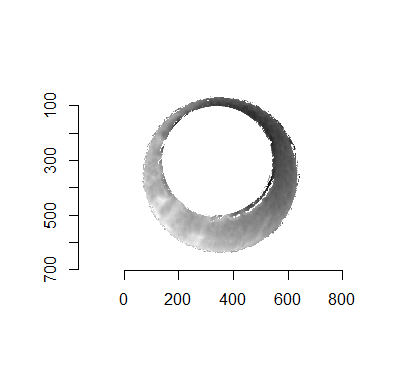
\includegraphics[width=0.5\linewidth]{images/cartridge_cases/im1_original} 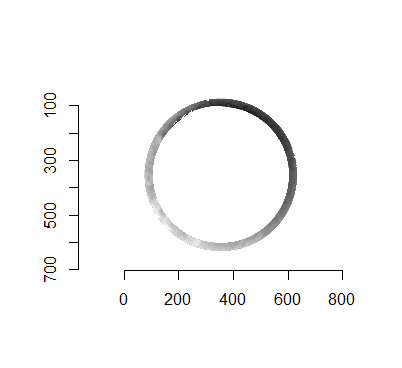
\includegraphics[width=0.5\linewidth]{images/cartridge_cases/im1_toroidalRegion} 

}

\caption{(Left) The original breech face impression scan image. (Right) A donut-shaped region cut out of the original image.}\label{fig:unnamed-chunk-15}
\end{figure}

By comparing such regions instead of the square cells, we would presumably only need to fill in a few missing value ``holes'' in the breech face impression scan rather than completely replacing a non-existent signal with an artificial one. In the near-future, I hope to finish up the pre-processing needed for this Congruent Matching Tori method by performing a polar transformation on these images to make them into strips that can easily be compared via an FFT.

Joe 9/12/19 Update: Before carving out toroidal regions from the two images we wish to compare, a fair amount of pre-processing needs to be completed. For example, the scans we work with begin with a considerable amount of auxiliary information, for example the firing pin impression, that we don't want to use in our comparisons. This isn't to say that firing pin impressions aren't useful to determine a match between two cartridge cases. In fact there is quite a lot of published research on how to compare two firing pin impressions. Rather, it is common practice to compare breech face impressions and firing pin impressions separately since it is difficult to scan both simultaneously. Thus, there are regions of a breech face impression scan that we want to remove so that the breech face impressions are more easily comparable. Below is an example of two breech face impression scans before processing.

\begin{figure}

{\centering 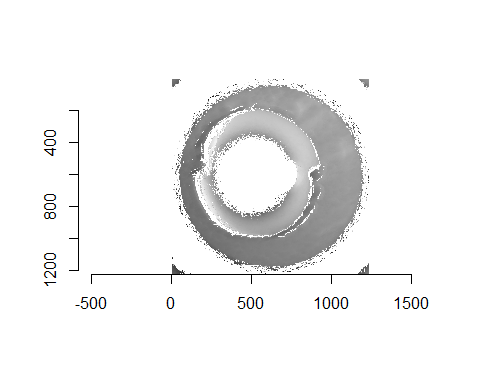
\includegraphics[width=0.5\linewidth]{images/cartridge_cases/im1_fullScan} 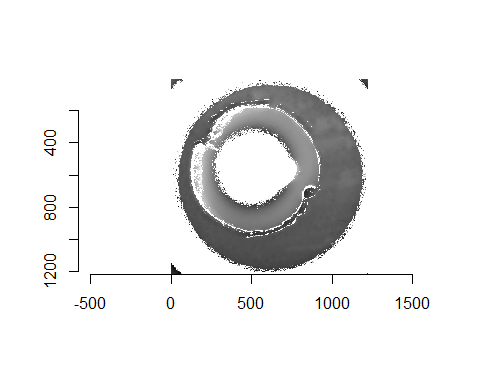
\includegraphics[width=0.5\linewidth]{images/cartridge_cases/im2_fullScan} 

}

\caption{Two cartridge case scans before pre-processing.}\label{fig:unnamed-chunk-16}
\end{figure}

There are a variety of techniques to segment an image into various parts. In image processing, common techniques are the Canny edge detector, which identifies edges of shapes in an image using image gradient techniques, and the Hough Transform, which can detect a variety of geometrical shapes in an image. The Hough Transform is what is used to segment the cartridge case images used in the previous section. However, we've found that the use of a Hough Transform doesn't extract the ``breech face signal'' from an image as other techniques. Namely, the breech face can be effectively extracted using the RANSAC (Random sample consensus) method that iteratively fits a plane to a set of data until it settles upon a consensus-based ``bulk'' of the data. In the case of these cartridge case scans, the bulk of the data should predominantely be distributed around the mode height value. That is, the breech face impression. Once we've fit this plane to the breech face impression, we can extract the residuals of the fit to better accentuate the markings left in the cartridge case base by a firearm's breech face. Below is an example of the residuals left after fitting a RANSAC plane to two cartridge case scans above. In the example below, we grab any residuals less than 20 microns in magnitude.

\begin{figure}

{\centering 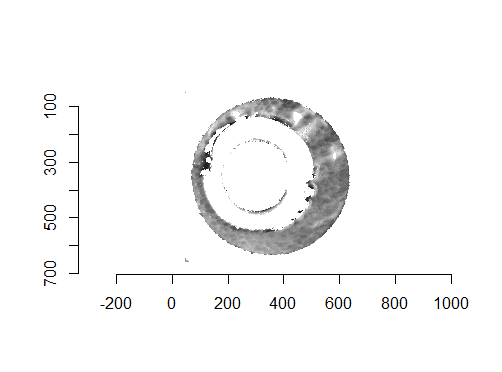
\includegraphics[width=0.5\linewidth]{images/cartridge_cases/im1_ransacResiduals} 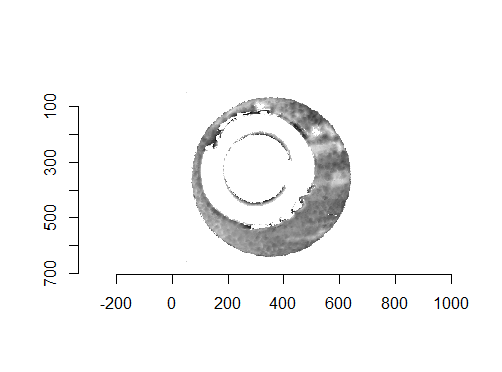
\includegraphics[width=0.5\linewidth]{images/cartridge_cases/im2_ransacResiduals} 

}

\caption{Residual values of a RANSAC plane fit to the two cartridge case scans shown above.}\label{fig:unnamed-chunk-17}
\end{figure}

Although these two images are of two different cartridge cases, you can hopefully see that one looks very much like a rotated version of the other. These two cartridge case scans are in fact fired from the same gun (known matches), so it's a good thing that they look so similar. We've now removed quite a bit of the unwanted regions of the original scans. However, there are still some areas of the image (e.g., the faint circular region of pixels in the center of the breech face scan) that just so happened to be close to the fitted plane and thus were brought along in the residual extraction. There are a few ways that we can clean up these last few areas. One is to use two Hough Transforms to detect the inner and outer circles of the breech face impression and filter out any pixels outside of the region between these two circles. The biggest issue with using a Hough Transform is that it must be given the radius of the circle that it is to search for in the image as an argument. That is, we need to know the radius of the breech face impression that we haven't yet identified in order to identify the breech face impression. Instead, we can dilate/erode (or vice-versa) the pixels in the image to remove the remaining ``speckle'' in the image. Below is an example of of the breech face impressions cleaned via a dilation/erosion procedure.

\begin{figure}

{\centering 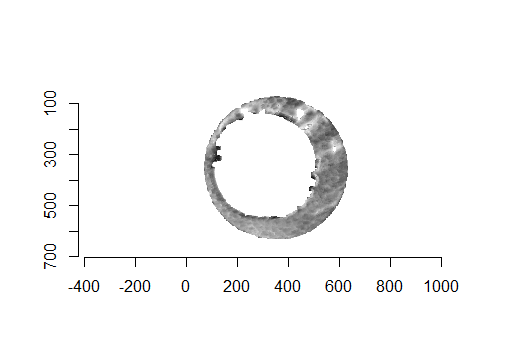
\includegraphics[width=0.5\linewidth]{images/cartridge_cases/im1_maskFiltered} 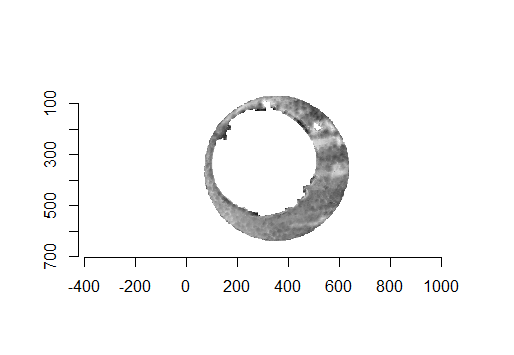
\includegraphics[width=0.5\linewidth]{images/cartridge_cases/im2_maskFiltered} 

}

\caption{The selected breech face impressions based on dilation and erosion.}\label{fig:unnamed-chunk-18}
\end{figure}

The final step in the pre-processing is to align the two images in some consistent fashion. Luckily, the firing pin impression ring that's left after performing the above dilation/erosion provides us with some idea of how to align the breech face impressions. The location of the firing ring impression in the breech face impression provides us with an indicator of where the cartridge case was located relative to the firing pin when it was sitting in the barrel. So aligning two cartridge cases so that their firing pin impression rings align will ensure that, at the very least, the breech face impression left on the cartridge case is horizontally/vertically aligned if not rotationally aligned.

\hypertarget{modified-chumbley-non-random}{%
\subsection{Modified Chumbley non-random}\label{modified-chumbley-non-random}}

\hypertarget{land-to-land-scores}{%
\subsubsection{Land-to-land scores}\label{land-to-land-scores}}

\hypertarget{bullet-to-bullet-scores}{%
\subsubsection{Bullet-to-bullet scores}\label{bullet-to-bullet-scores}}

Ganesh: In this method we extend the modified chumbley non-random method from land-to-land scoring to bullet-to-bullet scoring.

\hypertarget{analysis-of-results}{%
\section{Analysis of Results}\label{analysis-of-results}}

\hypertarget{communication-of-results-and-methods}{%
\section{Communication of Results and Methods}\label{communication-of-results-and-methods}}

The results are communicated through an interactive user interface. The first part of this interface lets you add all the bullets, barrels and lands for which the random forest and other scores are to be computed. A preliminary diagnostic of the orientations and dimensions of the lands tell us, if we can proceed safely to extraction of markings and then to cross-comparisons.

After this step, we can apply any sampling or interpolation needed on the land images, all these operations can be batched to the entire set of comparisons under consideration. Then we can make transformations like rotation, transpose etc on a sample image, visualize the results, and since we are dealing with conforming orientation and dimensions of lands present in the entire set, we can batch the transformations.

We extract markings, locate grooves, align signatures, and generate cross-comparison results. Each step is notified in UI and all steps are logged.

The scores and results are then communicated through an interactive visualization. We first interact at the top most level where we have bullet-to-bullet scores for all the cross-comparisons presented in a grid. We can select one comparison at a time which would generate a second level of grid visualization that shows the land-to-land scores for all 36 comparisons within a bullet. Interacting with this visualization, we can now pull up score tables, profiles, location of grooves, aligned signatures and raw images.

The framework of interactions, allows for validation of classification recommended by the RF model as well as gives an opportunity to critically asses, identify the cause and diagnose any problems encountered in the bullet matching pipeline.

\begin{figure}

{\centering 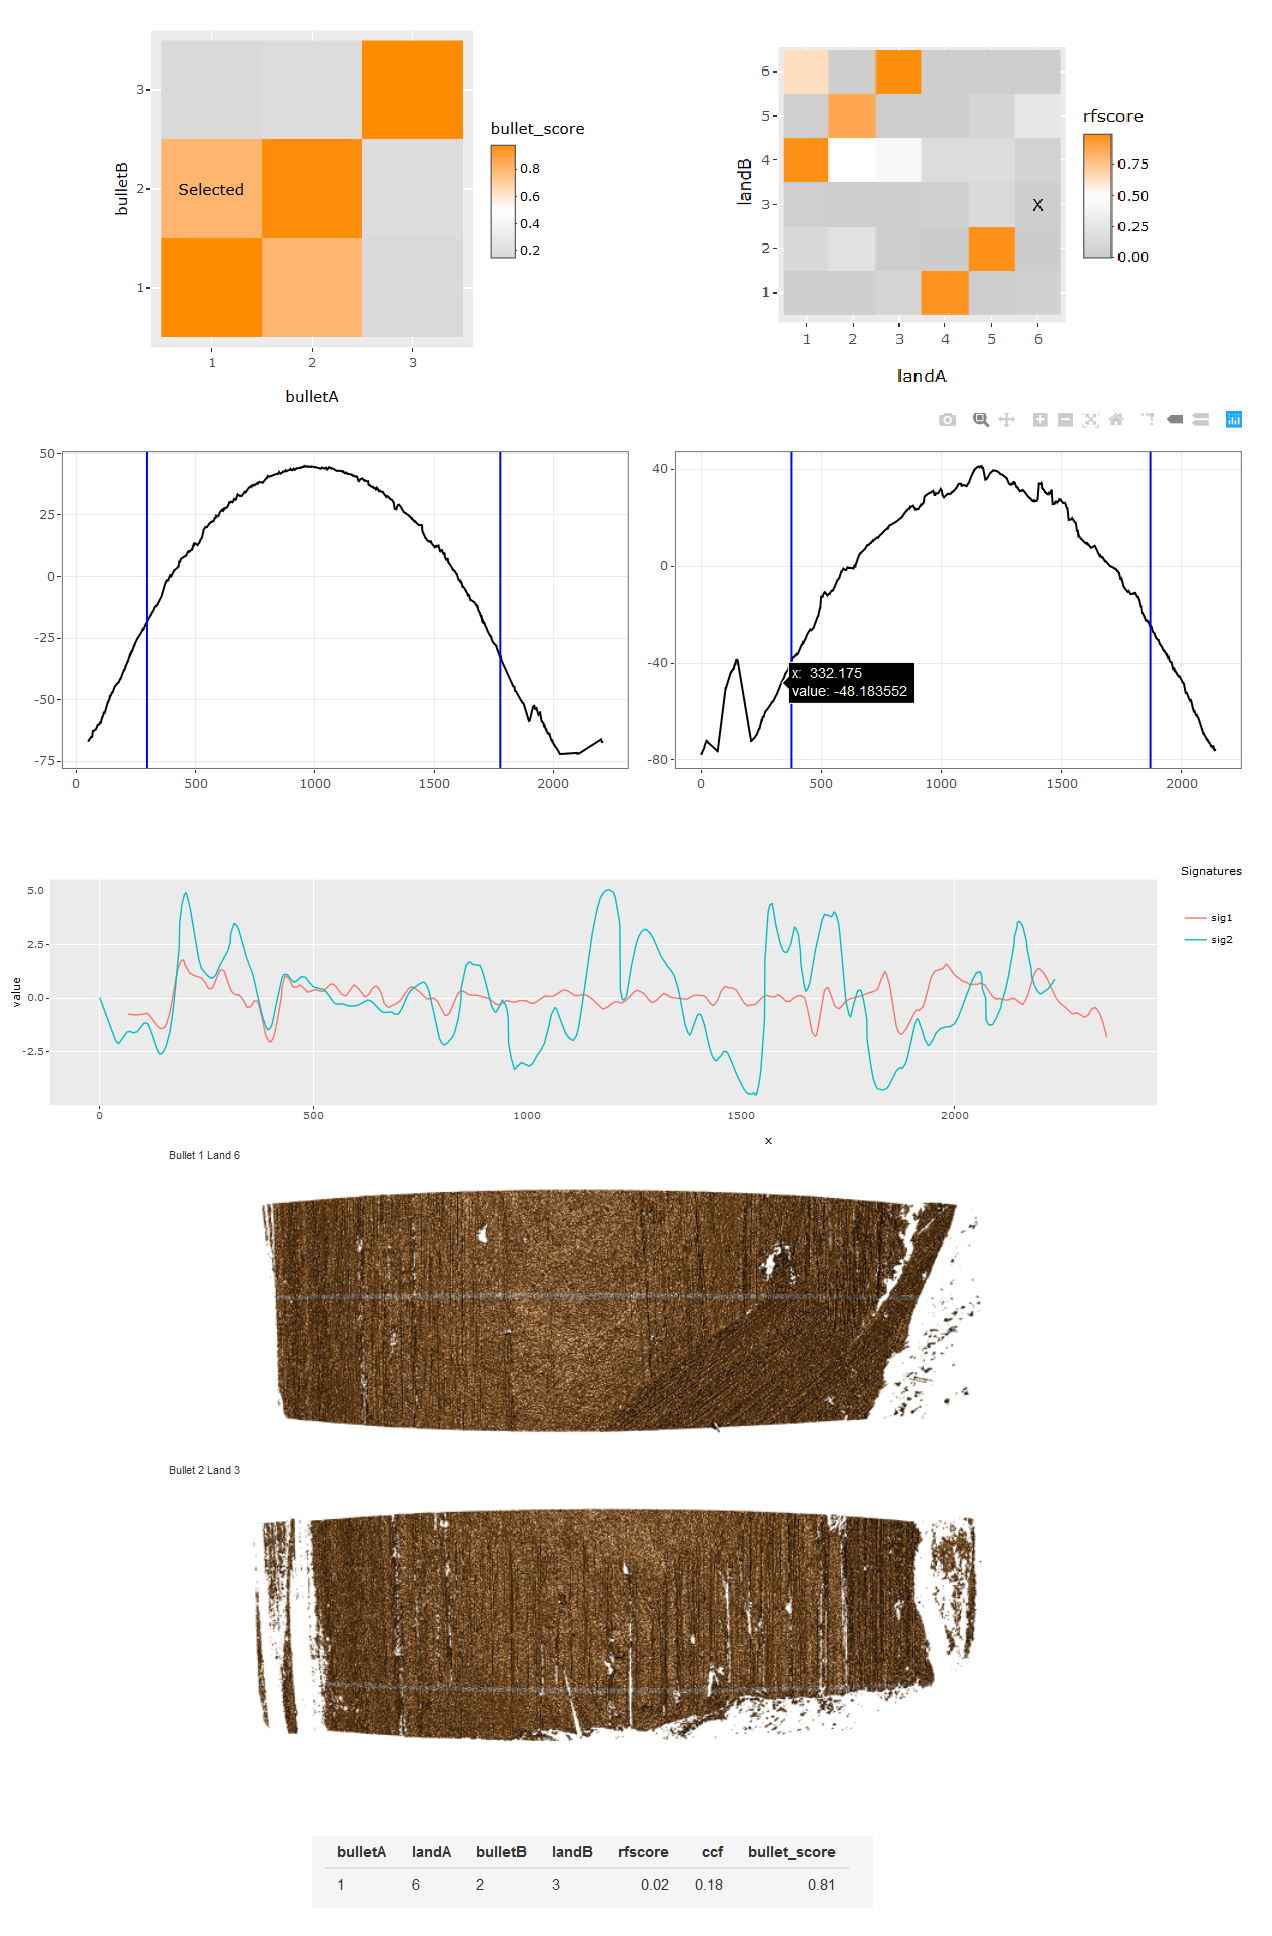
\includegraphics[width=0.5\linewidth]{images/bullets/gan-app2_consolidated} 

}

\caption{An instance of the interactive visualizations for communicating results}\label{fig:unnamed-chunk-19}
\end{figure}

\hypertarget{conference-presentations}{%
\subsection{Conference Presentations}\label{conference-presentations}}

\hypertarget{american-academy-of-forensic-sciences}{%
\subsubsection{American Academy of Forensic Sciences}\label{american-academy-of-forensic-sciences}}

\begin{itemize}
\item
  ``Validation Study on Automated Groove Detection Methods in 3D Bullet Land Scans''

  \begin{itemize}
  \tightlist
  \item
    February 2019\\
  \item
    Authors: Kiegan Rice, Ulrike Genschel, Heike Hofmann
  \item
    Presentation given by Kiegan Rice
  \end{itemize}
\end{itemize}

\hypertarget{association-of-firearms-and-toolmark-examiners-annual-training-seminar}{%
\subsubsection{Association of Firearms and Toolmark Examiners Annual Training Seminar}\label{association-of-firearms-and-toolmark-examiners-annual-training-seminar}}

\begin{itemize}
\item
  Heike's talk
\item
  ``Reproducibility of Automated Bullet Matching Scores Using High-Resolution 3D LEA Scans''

  \begin{itemize}
  \tightlist
  \item
    May 2019
  \item
    Authors: Kiegan Rice, Ulrike Genschel, Heike Hofmann
  \item
    Presentation given by Kiegan Rice
  \end{itemize}
\end{itemize}

\hypertarget{joint-statistical-meetings}{%
\subsubsection{Joint Statistical Meetings}\label{joint-statistical-meetings}}

\begin{itemize}
\item
  "A non-parametric test for matching bullet striations: extending the chumbley score for bullet-to-bullet matching

  \begin{itemize}
  \tightlist
  \item
    July 2019
  \item
    Authors:Ganesh Krishnan, Heike Hofmann
  \item
    Talk given by Ganesh Krishnan
  \end{itemize}
\item
  ``Repeatability and reproducibility of automated bullet comparisons using high-resolution 3D scans''

  \begin{itemize}
  \tightlist
  \item
    July 2019
  \item
    Authors: Kiegan Rice, Ulrike Genschel, Heike Hofmann
  \item
    Poster presented by Kiegan Rice
  \end{itemize}
\end{itemize}

\hypertarget{miscellaneous}{%
\subsubsection{Miscellaneous}\label{miscellaneous}}

\begin{itemize}
\item
  10th International Workshop on Statistics and Simulation in Salzburg, Austria, September 2019

  \begin{itemize}
  \tightlist
  \item
    ``Reproducibility of High-Resolution 3D Bullet Scans and Automated Bullet Matching Scores''

    \begin{itemize}
    \tightlist
    \item
      Authors: Kiegan Rice, Ulrike Genschel, Heike Hofmann
    \item
      Poster presented by Kiegan Rice, won 2nd Springer Poster Award\\
    \end{itemize}
  \item
    ``Case Study Validations of Automatic Bullet Matching''

    \begin{itemize}
    \tightlist
    \item
      Authors: Heike Hofmann, Susan VanderPlas
    \item
      Presentation given by Alicia Carriquiry
    \end{itemize}
  \end{itemize}
\end{itemize}

\hypertarget{people-involved}{%
\section{People involved}\label{people-involved}}

\hypertarget{faculty}{%
\subsection{Faculty}\label{faculty}}

\begin{itemize}
\tightlist
\item
  Heike Hofmann
\item
  Susan VanderPlas
\end{itemize}

\hypertarget{graduate-students}{%
\subsection{Graduate Students}\label{graduate-students}}

\begin{itemize}
\tightlist
\item
  Ganesh Krishnan
\item
  Kiegan Rice
\item
  Nate Garton
\item
  Charlotte Roigers
\item
  Joe Zemmels
\item
  Yawei Ge
\end{itemize}

\hypertarget{undergraduates}{%
\subsection{Undergraduates}\label{undergraduates}}

\begin{itemize}
\tightlist
\item
  Talen Fisher (fix3p)
\item
  Andrew Maloney
\item
  Mya Fisher, Allison Mark, Connor Hergenreter, Carley McConnell, Anyesha Ray (scanner)
\end{itemize}

\hypertarget{handwriting}{%
\chapter{Handwriting}\label{handwriting}}

We describe our methods for going about the handwriting project here.

\hypertarget{glass}{%
\chapter{Glass}\label{glass}}

\hypertarget{shoes}{%
\chapter{Shoes}\label{shoes}}

\hypertarget{longitudinal}{%
\section{Longitudinal Shoe Study}\label{longitudinal}}

\href{https://github.com/CSAFE-ISU/Longitudinal_Shoe_Study}{Github repository}

\hypertarget{paper-describing-the-database}{%
\subsection{Paper describing the database}\label{paper-describing-the-database}}

\href{https://github.com/CSAFE-ISU/Longitudinal_Shoe_Study/tree/master/Paper}{Paper subdirectory of Github repository}

Goal:

\begin{itemize}
\tightlist
\item
  Describe experiment
\item
  Describe database function
\item
  Publicize data for analysis by others in the community
\end{itemize}

\hypertarget{lss-paper-methods}{%
\subsubsection*{Methods and Data Description}\label{lss-paper-methods}}
\addcontentsline{toc}{subsubsection}{Methods and Data Description}

Methods and data description handed off to Alicia for editing

\hypertarget{lss-paper-analysis}{%
\subsubsection*{Data Analysis Tools}\label{lss-paper-analysis}}
\addcontentsline{toc}{subsubsection}{Data Analysis Tools}

\begin{itemize}
\tightlist
\item
  Working with the \texttt{EBImage} package - very fast processing of images
\end{itemize}

\hypertarget{lss-paper-analysis-film}{%
\paragraph{Film and Powder Images}\label{lss-paper-analysis-film}}
\addcontentsline{toc}{paragraph}{Film and Powder Images}

Analysis Summary: Create a mask via thresholding, clean it up, fill in mask holes, creating a shoe ``region'' mask. Apply this mask to the image, replacing any pixels outside the mask with the median background pixel. Additional thresholding and normalization can be applied if a binary image is more desireable.

\begin{enumerate}
\def\labelenumi{\arabic{enumi}.}
\item
  Create threshold mask

  \begin{enumerate}
  \def\labelenumii{\alph{enumii}.}
  \tightlist
  \item
    Blur image (circular/gaussian blur, diameter 15)\\
  \item
    Invert the image\\
  \item
    Threshold image (adaptive threshold, 10 x 10 region, keep anything with an average higher than 0.025 from the mean)\\
  \item
    Create mask\\
    Default parameters selected by visually screening several shoes:
    (default parameters rad1 = 5, rad2 = {91}, proportion = 1.5*area of rad2 in px/area of image in px)\\

    \begin{enumerate}
    \def\labelenumiii{\arabic{enumiii}.}
    \tightlist
    \item
      erode mask image (circle, diameter rad1)
    \item
      dilate mask image (circle, diameter rad2)
    \item
      label disjoint regions of the image
    \item
      prune small image regions (area \textless{} proportion parameter)
    \end{enumerate}
  \item
    Fill in mask holes\\
  \item
    Expand mask to capture entire shoe region

    \begin{enumerate}
    \def\labelenumiii{\arabic{enumiii}.}
    \tightlist
    \item
      set background color
    \item
      create dataframe of useful (non-background) pixels
    \item
      fill in holes and concave regions in mask, then expand by expand\_rad vertically and horizontally (similar to ``convex hull'', but with additional expansion radius)
    \end{enumerate}
  \end{enumerate}
\item
  Mask image to remove extra variability unrelated to the shoe\\
\item
  Threshold masked image?\\
  Con: Lose grey information; Pro: fully remove background\\
\item
  Compromise: Keep grey pixels from thresholded, masked image (e.g.~use 3. as a mask), then renormalize\\
\end{enumerate}

I've added the functions from last week to the \texttt{ShoeScrubR} package, which will hopefully contain methods for handling all of the different 2D shoe data from the longitudinal study.

Using that package, I tried the method out on a sequence of shoes over time to see what methods might best show wear. Each column shows a single left shoe over four timepoints. The shoes are the first 9 shoeIDs (e.g.~1 - 9).

Original

Cleaned\\

Cleaned and Thresholded

Even with the cleaning methods\ldots{} there is a lot of extra noise.

Next step: templating!

Basic framework:

Create a template for each size and model combination
(using GIMP - if I could automate this, I wouldn't need the template 🙄

Intelligently brute force angle and position of template\\
Goal: Maximize the number of black pixels in the image within the template region

\begin{enumerate}
\def\labelenumi{\arabic{enumi}.}
\item
  Start with an image and a template mask
\item
  Blur, normalize, invert, and threshold the image\\
\item
  Naively align the ``centers'' of the two images (avg of white pixel row/cols). To make this calculation comparable, do some very crude dilation/erosion (that may or may not generalize that well 😭) to fill in the image a bit.\\
  ~\\
  Then make the aligned center the actual center of the image via padding. (This is the 1st time we have modified the actual image beyond thresholding and color changes).
\item
  Create a new mask to sample the image (and the mask) radially.\\
  ~\\
  Create multiple radial masks, each offset slightly; optimize over the intersection (\# pixels or average pixel intensity) to get a coarse alignment angle.
\item
  Brute force for finer alignment.
\item
  Remove anything not in the mask region.
\end{enumerate}

Modified from \citep{kimGrayscaleTemplateMatchingInvariant2007}

\hypertarget{lss-paper-analysis-wear}{%
\paragraph{Wear Characterization}\label{lss-paper-analysis-wear}}
\addcontentsline{toc}{paragraph}{Wear Characterization}

Ideas:

\begin{itemize}
\tightlist
\item
  average intensity of cleaned image
\item
  length of border/edges detected
\end{itemize}

\hypertarget{connor}{%
\section{Passive Shoe Recognition}\label{connor}}

\#\#\#CoNNOR: Convolutional Neural Network for Outsole Recognition\#\#

\textbf{Project Overview}

\begin{itemize}
\tightlist
\item
  Label images of shoes according to geometric classification scheme
\item
  Use convolutional base of pretrained CNN VGG16 and train a new classifier on labeled features
\item
  Eventually, acquire real data passively and use CoNNOR to assess feature similarities and frequencies
\end{itemize}

\href{https://lib.dr.iastate.edu/creativecomponents/264/}{Link to submitted Creative Component on CoNNOR}

\href{https://github.com/srvanderplas/CoNNORFSI}{Github repository for paper submitted to Forensic Science International}

\textbf{Exploring new directions:}

\begin{itemize}
\tightlist
\item
  Truncate convolutional base and train random forest on features

  \begin{itemize}
  \tightlist
  \item
    Could replace fully connected layers of neural net as classifier
  \item
    Importance score can filter/reduce the number of features
  \item
    \emph{Block 4 random forest training terminated after one week :( }
  \item
    \emph{Block 5 currently training for two different random forest packages (randomForest and ranger)}
  \item
    \emph{If new models take more than 1-2 weeks, will look into subsampling techniques.}
  \end{itemize}
\item
  \emph{Spatial integration}

  \begin{itemize}
  \tightlist
  \item
    \emph{Model is currently set up to take in 256x256 pixels}
  \item
    \emph{Try taking in full shoe using a sliding window of size 256x256}
  \item
    \emph{View class predictions spatially}
  \end{itemize}
\item
  Fully convolutional networks (FCNs)

  \begin{itemize}
  \tightlist
  \item
    Unsupervised segmentation to assess current classification scheme
  \item
    Handle whole shoe image of any size (instead of only 256x256 pixel images)
  \end{itemize}
\end{itemize}

\textbf{References for CNNs and FCNs}

\href{https://stats.stackexchange.com/questions/266075/patch-wise-training-and-fully-convolutional-training-in-fully-convolutional-neur}{Stack Exchange post explaining patchwise training}

\href{https://ieeexplore.ieee.org/abstract/document/6338939}{``Learning Hierarchical Features for Scene Labeling''}: describes an application of multi-scale CNNs and image pyramids

\href{http://citeseerx.ist.psu.edu/viewdoc/summary?doi=10.1.1.56.8646}{``Pyramid methods in image processing''}: classic paper from 1984 explaining pyramid methods

\href{https://people.eecs.berkeley.edu/~jonlong/long_shelhamer_fcn.pdf}{``Fully Convolutional Networks for Semantic Segmentation''}

\href{https://arxiv.org/pdf/1711.08506.pdf}{``W-Net: A Deep Model for Fully Unsupervised Image Segmentation''}

\hypertarget{maxclique}{%
\section{Maximum Clique Matching}\label{maxclique}}

\hypertarget{cocoa}{%
\section{Project Tread (formerly Cocoa Powder Citizen Science)}\label{cocoa}}

Project Tread, modified from \href{https://www.dundee.ac.uk/leverhulme/citizenscience/details/sole-searching.php}{Leverhulme Institute's Sole Searching}, is a developing CSAFE project with the goals of engaging community participation in forensic research and acquiring shoe print data that may be useful in future analyses.

In progress:

\begin{itemize}
\tightlist
\item
  Review \href{https://forensicstats.org/project-tread/}{procedures} and IRB documents written by James
\item
  Perhaps modify procedures, then bribe some friends into helping me test them :)

  \begin{itemize}
  \tightlist
  \item
    Test for length, clarity, ease, etc.
  \end{itemize}
\item
  Be involved in set up of data collection site (through CSSM)
\end{itemize}

\hypertarget{d-shoe-recognition}{%
\section{3d Shoe Recognition}\label{d-shoe-recognition}}

The set up

What we have tried

What we are doing now
- Transforming the mesh objects to points aligned by the center of mass to overlay them detecting difference.
- Problems
- Isnt aligning properly as you can see
- Next
- angle transformations

\hypertarget{theoretical-foundations}{%
\chapter{Theoretical foundations}\label{theoretical-foundations}}

\hypertarget{nates-updates-952019}{%
\section{Nate's Updates 9/5/2019}\label{nates-updates-952019}}

\begin{itemize}
\tightlist
\item
  Currently in Virginia
\item
  RA for this semester (year?) is under Danica
\item
  \textbf{Central Goals}:

  \begin{itemize}
  \tightlist
  \item
    continue work started by Danica and Peter Vergeer on the analysis of likelihood ratios
  \item
    study the differences between specific source (SS) and common source (CS) likelihood ratios (LRs) in an information theoretic way
  \item
    does the CS or SS LR have more ``information''?
  \item
    can be the CS or SS hypotheses (prosecution or defense) be formally compared in terms of being easier to ``prove'' or ``disprove''?
  \end{itemize}
\item
  \textbf{Basic Setup}

  \begin{itemize}
  \tightlist
  \item
    \(H_p\), \(H_d\) are CS prosecution and defense hypotheses upon which we will place priors\\
  \item
    \(A\) and \(B\) are discrete r.v.'s representing two ``sources'' of evidence

    \begin{itemize}
    \tightlist
    \item
      distributions for \(A\) and \(B\) defined conditionally based on the hypothesis
    \item
      SS hypothesis is represented by the conditional random variable \(H_p|A\)
    \end{itemize}
  \item
    \(X\) is data coming from \(A\), \(Y\) is data coming from \(B\)
  \item
    compare information contained in \((X,Y)\) about \(H_p\) and \(H_p|A\)

    \begin{itemize}
    \tightlist
    \item
      this is what I'm working on now
    \item
      important quantities:

      \begin{itemize}
      \tightlist
      \item
        Kullback-Leibler divergences, entropy, mutual information
      \end{itemize}
    \end{itemize}
  \end{itemize}
\end{itemize}

\hypertarget{nates-updates-9122019}{%
\section{Nate's Updates 9/12/2019}\label{nates-updates-9122019}}

\begin{itemize}
\tightlist
\item
  Assume \(p(X,Y,A,B,H) = p(X,Y|A,B)p(B|A,H)p(A|H)p(H)\)
\item
  Entropy: \(E(X) = \int -p(x)\log p(x) dx\)

  \begin{itemize}
  \tightlist
  \item
    ``average amount of information gained through observation of \(X = x\) "

    \begin{itemize}
    \tightlist
    \item
      low entropy \(\implies\) better able to predict outcome
    \item
      \(\mathcal{E}(H|X,Y) \geq \mathcal{E}(H|X,Y,A)\)

      \begin{itemize}
      \tightlist
      \item
        Common source (posterior) entropy is greater than specific source
      \end{itemize}
    \end{itemize}
  \item
    Mutual Information: \(\mathcal{I}(X;Y) = \mathcal{E}(X) - \mathcal{E}(X|Y)\)

    \begin{itemize}
    \tightlist
    \item
      \(\mathcal{I}(X;Y) = KL(p(X,Y)||p(X),p(Y)) \geq 0\)
    \end{itemize}
  \end{itemize}
\end{itemize}

\hypertarget{outreach-activities}{%
\chapter{Outreach activities}\label{outreach-activities}}

CSAFE has several ongoing outreach projects.

\hypertarget{book-on-forensic-science-and-statistics}{%
\section{Book on Forensic Science and Statistics}\label{book-on-forensic-science-and-statistics}}

Project members:

\begin{itemize}
\tightlist
\item
  Kiegan Rice\\
\item
  Alicia Carriquiry\\
\item
  Hal Stern (UCI)
\end{itemize}

General book outline:

\begin{itemize}
\tightlist
\item
  Chapter 1: Introduction\\
\item
  Chapter 2: Analysis of Forensic Evidence

  \begin{itemize}
  \tightlist
  \item
    Drafted. In the editing stage.
  \end{itemize}
\item
  Chapter 3: The Path to the Witness Stand

  \begin{itemize}
  \item
    Drafted. In the editing stage.
  \end{itemize}
\item
  Chapter 4: Communicating Evidence in the Courtroom

  \begin{itemize}
  \tightlist
  \item
    Not drafted. In the writing stage.
  \end{itemize}
\item
  Chapter 5: Conclusions
\end{itemize}

\bibliography{book.bib,packages.bib}


\end{document}
